\documentclass[journal,twoside,web]{ieeecolor}
\pdfobjcompresslevel=0   % disable object-stream compression (avoids buffer overflow)
\pdfcompresslevel=9      % compress streams (keeps file size reasonable)
\pdfminorversion=5       % lower PDF version compatibility

\usepackage{jsen}
\usepackage{cite}
\usepackage{amsmath,amssymb,amsfonts}
\usepackage{graphicx}
\usepackage{caption}
\usepackage{subcaption}
\usepackage{textcomp}
\usepackage{float}
\usepackage{wrapfig}
\usepackage{tabularx}
\usepackage{multirow}
\usepackage{siunitx}
\usepackage{booktabs}
\usepackage[table,xcdraw]{xcolor}
\usepackage[english]{babel}
\usepackage[utf8]{inputenc}
\usepackage{algorithm}
\usepackage{algorithmic}
\usepackage{pifont}
\usepackage{hyperref}
\usepackage{makecell}

\pdfobjcompresslevel=0
\pdfminorversion=5

\newcommand{\cmark}{\ding{51}}%
\newcommand{\xmark}{\ding{55}}%

\def\BibTeX{{\rm B\kern-.05em{\sc i\kern-.025em b}\kern-.08em
    T\kern-.1667em\lower.7ex\hbox{E}\kern-.125emX}}
\markboth{\journalname, }
{Author \MakeLowercase{\textit{et al.}}: Preparation of Papers for IEEE TRANSACTIONS and JOURNALS (February 2017)}
\definecolor{abstractbg}{rgb}{0.89804,0.94510,0.83137}
\setlength{\fboxrule}{0pt}
\setlength{\fboxsep}{0pt}

\begin{document}
\title{Thermal-Security-YOLO: Hybrid Dilated Channel Attention for Thermal Transit Surveillance and Edge Hardware Energy Profiling}

\author{Satya Mohit, Bethi Pardhasaradhi, \IEEEmembership{Member, IEEE},
and Linga Reddy Cenkeramaddi, \IEEEmembership{Senior Member, IEEE}
\thanks{Compiled on \today.}
\thanks{Satya Mohit, Bethi Pardhasaradhi, and Linga Reddy Cenkeramaddi are with the autonomous and cyber-physical systems (ACPS) research group, Department of Information and Communication Technology (ICT), University of Agder, Campus Grimstad, Jon Lilletuns Vei 9, 4879 Grimstad, Norway (e-mail: satyam@uia.no, pardhasaradhi.bethi@uia.no, linga.cenkeramaddi@uia.no).}
}

\IEEEtitleabstractindextext{%
\fcolorbox{abstractbg}{abstractbg}{%
\begin{minipage}{\textwidth}%
\begin{wrapfigure}[11]{r}{3in}%
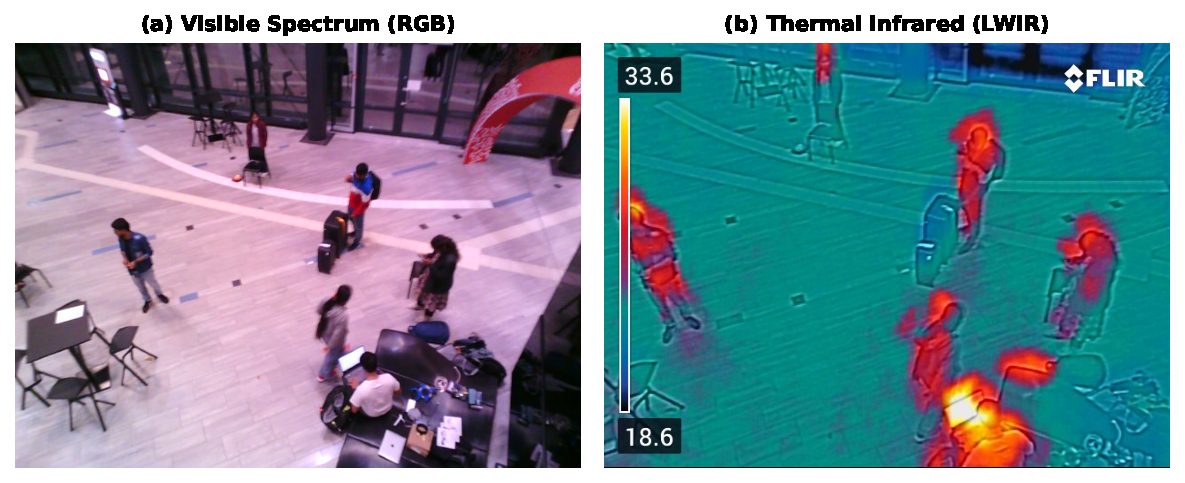
\includegraphics[width=2.9in]{yolo_thermal_front.pdf}%
\end{wrapfigure}%
\begin{abstract}
Automated video surveillance in high-throughput transit hubs, such as airport terminals, railway stations, and multi-modal transit corridors, requires robust 24/7 perception that functions reliably irrespective of optical illumination while strictly preserving personal privacy. Long-wave infrared (LWIR) thermal sensors provide illumination-invariant sensing and inherent privacy preservation by imaging radiometric temperature differentials rather than identifying visual textures. However, deploying object detectors on thermal surveillance streams poses severe challenges: diffuse thermal boundaries, lack of optical surface textures, subtle temperature contrast between carried items and human bodies, and the critical security requirement of identifying both mobile entities (\textit{Person}, \textit{Trolley}, \textit{Bag}) and stationary safety hazards (\textit{Unattended Anomaly}). Furthermore, smart camera installations demand execution on severely resource-constrained edge computing hardware. To address these challenges, this paper presents \textbf{Thermal-Security-YOLO}, a lightweight, thermally co-optimized detection framework tailored for transit security surveillance. We introduce a newly curated Thermal Security Surveillance dataset comprising 1,067 verified LWIR frames and 3,849 annotated instances across transit security classes. To overcome the receptive field limitations of standard convolutional kernels without parameter inflation, we propose \textbf{Hybrid Dilated ECA-YOLO}. The architecture selectively embeds dilated residual bottlenecks ($d=2$) in deeper feature stages ($P_4$, $P_5$) coupled with parameter-free 1D Efficient Channel Attention (ECA) to capture long-range contextual spatial relationships while avoiding early-stage gridding artifacts. Our model achieves \textbf{87.89\% mAP@50 and 64.73\% mAP@50--95} on the held-out test split with only \textbf{3.01\,M parameters and 8.1\,GFLOPs}. Crucially, it yields massive recall improvements on security-critical targets (+8.5pp for Person, +10.2pp for Bag, and +11.0pp for Unattended Anomaly) and out-localizes larger 11\,M+ parameter models (YOLOv8s, YOLO11s) while running 1.8$\times$ faster. Finally, we conduct empirical hardware deployment and in-line physical energy profiling using a laboratory-grade \textbf{Joulescope JS220 high-speed DC energy analyzer} (2\,MS/s) across a Waveshare ESP32-P4 dual-core RISC-V microcontroller (INT8 ESP-DL hardware 2D accelerator: 2173.7\,ms, 1.23\,W, 18.1\,MB free PSRAM), a Raspberry Pi 5 SBC (673.7\,ms, 4.85\,W, 3268.8\,mJ/frame), and an NVIDIA Jetson AGX Xavier (7.71\,ms, 129.7\,FPS, 11.01\,W, achieving top energy efficiency at 11.78\,frames/Joule). These results validate our framework as a practical, energy-efficient solution for autonomous privacy-preserving transit security.
\end{abstract}

\begin{IEEEkeywords}
Thermal infrared sensing, object detection, security surveillance, transit hubs, unattended luggage anomaly, Efficient Channel Attention, dilated convolution, edge computing, RISC-V, ESP32-P4, Joulescope energy profiling.
\end{IEEEkeywords}
\end{minipage}}}
\maketitle

\section{Introduction}
\label{sec:introduction}

\begin{figure}[t]
\centering
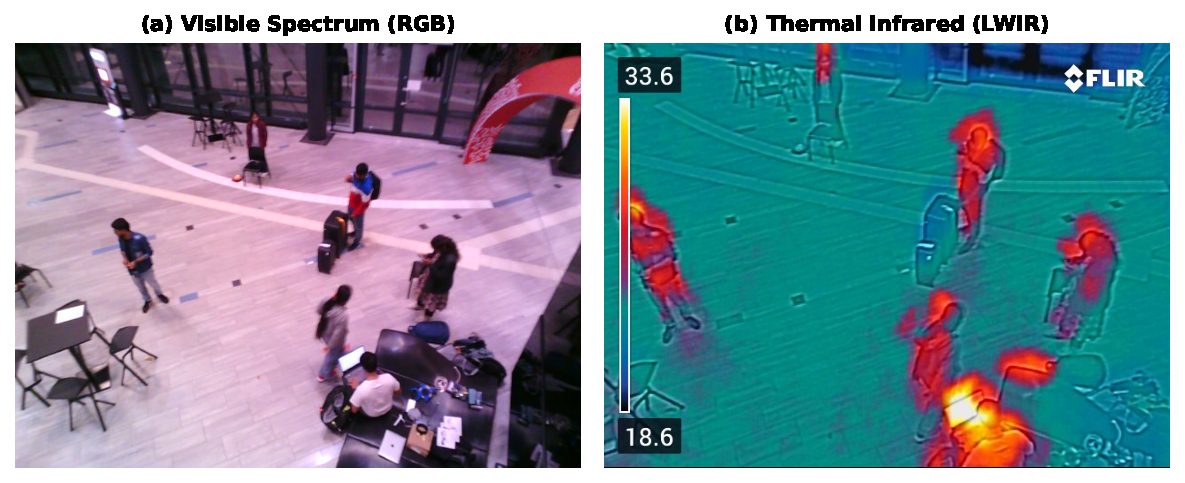
\includegraphics[width=\columnwidth]{rgb_thermal_side_by_side.pdf}
\caption{Visual comparison between visible-spectrum (RGB) and long-wave infrared (LWIR) sensing modalities in a transit concourse: (a) optical RGB camera captures identifiable facial identities and fine clothing textures while suffering from specular floor glare and sensitivity to ambient light; (b) LWIR thermal imaging detects radiated body heat and temperature differentials, inherently protecting personal privacy while providing robust 24/7 detection of pedestrians, luggage, and metal baggage trolleys regardless of ambient illumination.}
\label{fig:rgb_thermal_comparison}
\end{figure}

Automated surveillance systems deployed in high-throughput transit hubs---such as international airport terminals, railway concourses, and metro transit stations---play a vital role in ensuring public safety, crowd flow optimization, and anomaly detection~\cite{wilson2023recent,zhang2020traffic}. Conventional visual surveillance architectures rely predominantly on visible-spectrum (RGB) optical cameras. However, optical sensors suffer from fundamental limitations in complex real-world environments: their performance degrades severely under low-light night conditions, heavy artificial glare, abrupt shadows, backlighting through glass facades, and atmospheric obscuration such as smoke or steam~\cite{altay2022use}. Furthermore, as illustrated in Fig.~\ref{fig:rgb_thermal_comparison}, visible cameras capture identifiable facial traits and clothing textures, raising severe privacy and data protection concerns under strict regulatory frameworks such as the European General Data Protection Regulation (GDPR)~\cite{breland2021robust,guan2018daily}.

Thermal infrared (IR) sensors, specifically operating in the Long-Wave Infrared (LWIR) spectral band ($7.5\text{--}13.5\,\mu\text{m}$), provide an ideal sensing alternative. LWIR sensors detect passive radiant heat emitted directly by human bodies and physical objects rather than reflected ambient illumination. Consequently, thermal imaging is completely invariant to lighting conditions, operating with identical fidelity in pitch darkness, direct sunlight, and optical glare. Moreover, because thermal imagery captures thermal signatures rather than biometric surface pigmentation, it inherently preserves individual privacy, enabling continuous visual monitoring in sensitive public terminals without ethical or legal friction~\cite{wilson2023recent}.

Despite these compelling operational advantages, detecting security-critical objects in thermal surveillance imagery introduces formidable technical challenges:
\begin{enumerate}
    \item \textbf{Low Contrast and Diffuse Thermal Boundaries:} Long-wave radiation is inherently blurry and lacks high-frequency color or texture edges. In transit hubs, passengers frequently carry bags, pull rolling luggage, or navigate with airport baggage trolleys. Because metallic or synthetic luggage surfaces rapidly equilibrate with ambient indoor air while human bodies radiate warm body heat ($37^\circ\text{C}$), carried items often exhibit low radiometric contrast against background floors and human limbs.
    \item \textbf{Critical Unattended Luggage Anomaly Detection:} Identifying abandoned or unattended baggage items is one of the most critical security imperatives in transit facilities. While a bag held or carried by a walking passenger moves dynamically with the human heat signature, an unattended bag becomes a stationary, cooling radiometric anomaly detached from any thermal human core. Detecting such subtle spatial anomalies reliably without triggering crippling false alarm rates requires robust contextual spatial reasoning.
    \item \textbf{Severe Edge Deployment Constraints:} Real-world transit security architectures increasingly favor decentralized smart cameras or battery/PoE-powered edge sensing nodes to eliminate continuous, bandwidth-heavy video streaming to centralized servers~\cite{humes2023squeezed,okano2025edge}. These edge nodes often rely on resource-constrained embedded microcontrollers (e.g., RISC-V processors) or compact single-board computers (SBCs) with strict memory buffers (tens of megabytes) and milliwatt-scale power budgets. Standard lightweight object detectors (e.g., stock YOLOv8n) employ small $3\times3$ convolutional kernels that possess insufficient receptive fields to bind human bodies with distant trolley frames or subtle luggage contours. Conversely, heavy attention mechanisms, deformable convolutions, or transformer backbones incur severe memory and latency bottlenecks that cause out-of-memory (OOM) failures on embedded edge hardware~\cite{luo2025yolo,li2024yolo}.
\end{enumerate}

To overcome these coupled sensing, modeling, and edge execution challenges, this work introduces \textbf{Thermal-Security-YOLO}, a lightweight, thermally co-optimized object detection and edge execution framework tailored specifically for transit hub surveillance. 

We curate and annotate a specialized \textbf{Thermal Security Surveillance dataset} comprising 1,067 unique high-resolution LWIR frames and 3,849 object instances captured in realistic transit settings across four target classes: \textit{Person}, \textit{Trolley} (wheeled baggage carts), \textit{Bag} (carried luggage and backpacks), and \textit{Unattended Anomaly} (stationary abandoned luggage).

To maximize thermal discriminability without expanding model capacity, we propose \textbf{Hybrid Dilated ECA-YOLO}. Rather than inserting heavy spatial attention or computationally demanding deformable convolutions, we develop a stage-selective architecture that integrates dilated convolutions ($d=2$) within the bottleneck layers of deeper feature stages ($P_4$ and $P_5$), combined with 1D parameter-free Efficient Channel Attention (ECA)~\cite{wang2020eca}. The dilated bottleneck effectively expands the receptive field from $3\times3$ to $5\times5$ ($D_{\text{eff}}=5$), enabling the network to capture extended physical context (such as the geometric relationship between a passenger and their baggage cart) without adding parameters or downsampling fine spatial resolution. Dense convolutions ($d=1$) are preserved in early stages ($P_2, P_3$) to prevent high-frequency gridding artifacts on localized thermal gradients.

Furthermore, we conduct empirical hardware deployment and physical electrical profiling using an in-line laboratory-grade \textbf{Joulescope JS220 high-speed precision DC energy analyzer} sampling at 2\,MS/s. We benchmark our model alongside four state-of-the-art YOLO baselines (YOLOv8n, YOLOv8s, YOLO11n, YOLO11s) across three distinct hardware tiers: an ultra-low-power dual-core RISC-V microcontroller (Waveshare ESP32-P4 Nano running ESP-DL INT8 hardware 2D DMA acceleration), a single-board computer (Raspberry Pi 5 running multi-threaded CPU ONNX Runtime), and an embedded GPU platform (NVIDIA Jetson AGX Xavier running TensorRT FP16).

\textbf{Main Contributions of this Work:}
\begin{enumerate}
    \item \textbf{Thermal Security Surveillance Benchmark:} We curate and evaluate a dedicated LWIR thermal dataset comprising 1,067 frames and 3,849 instances capturing complex human--baggage interactions and unattended luggage anomalies in transit security settings.
    \item \textbf{Lightweight Hybrid Dilated ECA-YOLO Architecture:} We design a compact thermal detector (3.01\,M parameters, 8.1\,GFLOPs) that pairs stage-selective dilated residual bottlenecks ($d=2$ at $P_4, P_5$) with 1D adaptive Efficient Channel Attention. The model achieves 87.89\% mAP@50 and 64.73\% mAP@50--95 on the held-out test split, outperforming stock YOLOv8n (+4.48pp precision, +2.39pp mAP@50, +1.81pp mAP@50--95) and matching or outperforming 11\,M+ parameter models (YOLOv8s, YOLO11s).
    \item \textbf{Targeted Security Recall & Localization Gains:} Our architecture yields massive recall improvements on critical security targets: \textbf{+8.5pp for Person (66.4\%)}, \textbf{+10.2pp for Bag (89.7\%)}, and \textbf{+11.0pp for Unattended Anomaly (83.3\%)}, along with substantial tight localization improvements (+4.5pp mAP@50--95 on Person and +3.5pp on Unattended Anomaly), effectively mitigating thermal boundary blur.
    \item \textbf{Physical Joulescope Energy Profiling across Heterogeneous Edge Tiers:} We present rigorous empirical power, frame latency, energy-per-frame, and memory measurements using an in-line Joulescope JS220 across RISC-V microcontroller (ESP32-P4), ARM CPU (RPi 5), and Volta GPU (Jetson) platforms. Our model achieves top energy efficiency on GPU (11.78\,frames/Joule) and maintains 18.1\,MB of free PSRAM headroom on the microcontroller, where larger models induce near-OOM instability.
\end{enumerate}

\section{Thermal Security Dataset and Related Benchmarks}
\label{sec:dataset_and_related}

\subsection{Comparison with Existing Infrared Benchmarks}
As shown in Table~\ref{tab:dataset_comparison}, existing infrared object detection datasets have almost exclusively focused on automotive road scenes or military target tracking. The OSU Thermal Pedestrian database~\cite{davis2007background} pioneered static-camera surveillance evaluation but restricted annotations to a single monolithic pedestrian class. The KAIST Multispectral benchmark~\cite{choi2018kaist} and FLIR ADAS dataset~\cite{flir_adas_dataset} introduced paired RGB-thermal imagery for autonomous vehicle navigation, categorizing roadway objects such as cars, trucks, pedestrians, and cyclists. Other datasets such as CVC-14~\cite{gonzalez2016pedestrian}, LLVIP~\cite{jia2021llvip}, and M3FD~\cite{liu2022target} focused on low-light urban streets and multi-modal target fusion.

\begin{table*}[t]
\centering
\caption{Comparison of the Proposed Thermal Security Dataset with Existing Infrared Object Detection Benchmarks}
\label{tab:dataset_comparison}
\resizebox{\textwidth}{!}{%
\begin{tabular}{l c c l c c c}
\toprule
\textbf{Benchmark Dataset} & 
\textbf{Year} & 
\textbf{Modality} & 
\textbf{\makecell[c]{Target Domain /\\Surveillance Setting}} & 
\textbf{\makecell[c]{Pedestrian\\Detection}} & 
\textbf{\makecell[c]{Carried Luggage\\(Trolley, Bag)}} & 
\textbf{\makecell[c]{Unattended\\Anomaly}} \\
\midrule
OSU Thermal~\cite{davis2007background}    & 2005 & LWIR Thermal  & Static Campus Surveillance   & \cmark & \xmark & \xmark \\
KAIST Multispectral~\cite{choi2018kaist}   & 2018 & Thermal + RGB & Autonomous Driving (Roadway) & \cmark & \xmark & \xmark \\
FLIR ADAS~\cite{flir_adas_dataset}         & 2019 & Thermal + RGB & Autonomous Driving (Roadway) & \cmark & \xmark & \xmark \\
CVC-14~\cite{gonzalez2016pedestrian}       & 2016 & Thermal + RGB & Automotive Pedestrian Only   & \cmark & \xmark & \xmark \\
LLVIP~\cite{jia2021llvip}                  & 2021 & Thermal + RGB & Low-Light Pedestrian Urban   & \cmark & \xmark & \xmark \\
M3FD~\cite{liu2022target}                  & 2022 & Thermal + RGB & Multi-Scenario Target Track  & \cmark & \xmark & \xmark \\
\midrule
\textbf{Ours (Thermal Security)}           & \textbf{2026} & \textbf{LWIR Thermal} & \textbf{Transit Hub / Security Surveillance} & \textbf{\cmark} & \textbf{\cmark} & \textbf{\cmark} \\
\bottomrule
\end{tabular}%
}
\vspace{1ex}
{\raggedright \footnotesize \textit{Note}: \cmark\ indicates explicit class annotation; \xmark\ indicates absent or unannotated. While conventional benchmarks evaluate open roadways, our dataset uniquely targets high-throughput security facilities where pedestrians actively interact with carried luggage, baggage trolleys, and potential unattended anomaly objects.\par}
\end{table*}

None of these existing benchmarks address transit hub surveillance where passengers interact with carried baggage, push multi-tiered luggage trolleys, or where unattended items present potential safety hazards. The proposed Thermal Security Surveillance dataset bridges this critical gap.

\begin{figure}[t]
\centering
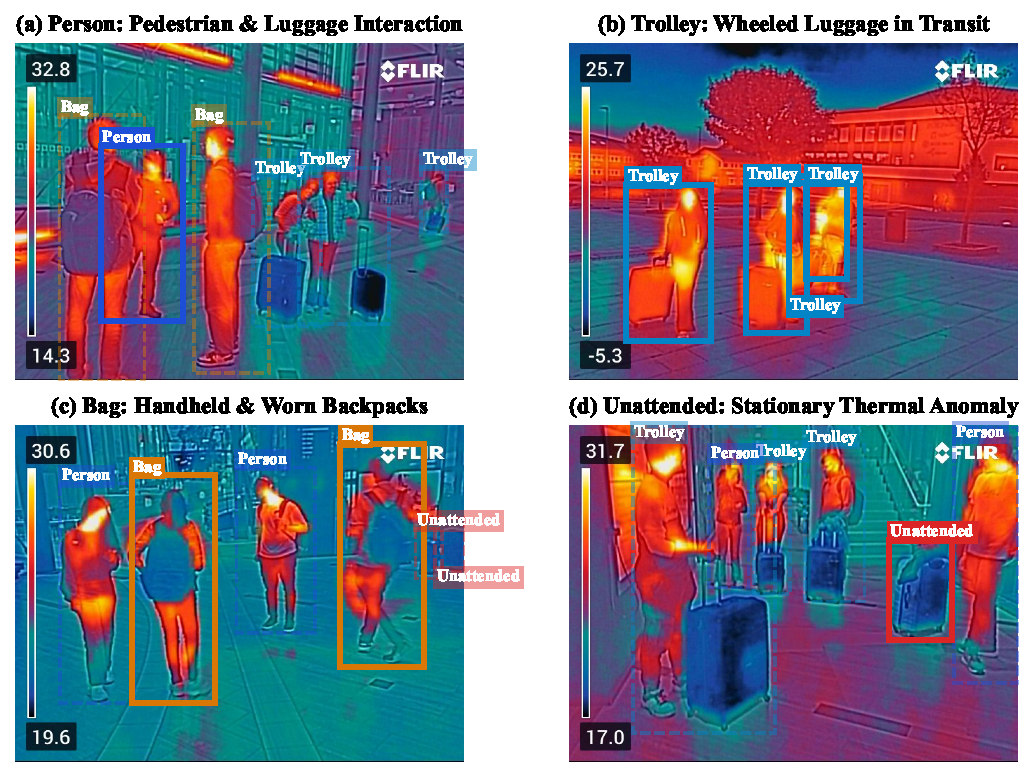
\includegraphics[width=\columnwidth]{fig1_dataset_samples.pdf}
\caption{Representative sample frames from the proposed Thermal Security Surveillance dataset, illustrating pedestrians interacting with baggage trolleys, carried luggage, and stationary unattended luggage anomalies under varied thermal contrast.}
\label{fig:dataset_samples}
\end{figure}

\subsection{Thermal Security Dataset Collection and Split Statistics}
Data acquisition was performed using calibrated FLIR Long-Wave Infrared (LWIR) sensors operating in the $7.5\text{--}13.5\,\mu\text{m}$ spectral bandwidth with a native resolution of $640\times512$ pixels. Cameras were mounted at elevated overhead surveillance vantage points ($2.5\text{--}4.0$\,m height) overlooking passenger concourses, check-in corridors, and baggage claim zones.

The dataset contains \textbf{1,067 unique thermal frames} comprising \textbf{3,849 precisely annotated bounding-box instances}. The four target classes are defined as follows:
\begin{enumerate}
    \item \textbf{Person (1,076 instances, 28.0\%):} Moving and stationary pedestrians, airport staff, and passengers traversing transit areas unassisted or in transit flow.
    \item \textbf{Trolley (2,145 instances, 55.7\%):} Metallic wheeled baggage carts, airport trolleys, and luggage pushcarts, either pushed by individuals or clustered in transit staging bays.
    \item \textbf{Bag (353 instances, 9.2\%):} Backpacks, suitcases, shoulder bags, and duffel bags held, carried, or pulled in direct physical contact with a walking person.
    \item \textbf{Unattended Anomaly (275 instances, 7.1\%):} Stationary, isolated baggage items, parcels, or luggage detached from any human handler for extended durations, representing potential security anomalies.
\end{enumerate}

\begin{table}[t]
\centering
\caption{Thermal Security Dataset Class Definitions and Instance Counts Across Data Splits}
\label{tab:dataset_distribution}
\small
\setlength{\tabcolsep}{2pt}
\renewcommand{\arraystretch}{1.15}
\begin{tabular}{lcccccc}
\toprule
\textbf{Class} & \textbf{Surveillance Context} & \textbf{Train} & \textbf{Val} & \textbf{Test} & \textbf{Total (\%)} \\
\midrule
\textbf{Person}     & Pedestrians \& individuals       & 742     & 237 & 97  & 1{,}076 (28.0\%) \\
\textbf{Trolley}    & Wheeled baggage carts            & 1{,}514 & 407 & 224 & 2{,}145 (55.7\%) \\
\textbf{Bag}        & Carried backpacks/luggage        & 250     & 64  & 39  & 353 (9.2\%) \\
\textbf{Unattended} & Stationary luggage anomaly       & 177     & 68  & 30  & 275 (7.1\%) \\
\midrule
\textbf{Total Inst.}& All bounding boxes               & 2{,}683 & 776 & 390 & 3{,}849 (100\%) \\
\textbf{Total Img.} & Unique thermal frames            & 746     & 213 & 108 & 1{,}067 (100\%) \\
\bottomrule
\end{tabular}
\end{table}

Table~\ref{tab:dataset_distribution} details the official train, validation, and held-out test splits. A strict 70\%/20\%/10\% image-level partitioning was enforced across unique recording sequences to prevent temporal data leakage. The held-out test split contains 108 frames and 390 ground-truth objects, serving as the benchmark for all evaluations in this paper.

\begin{figure*}[t]
\centering
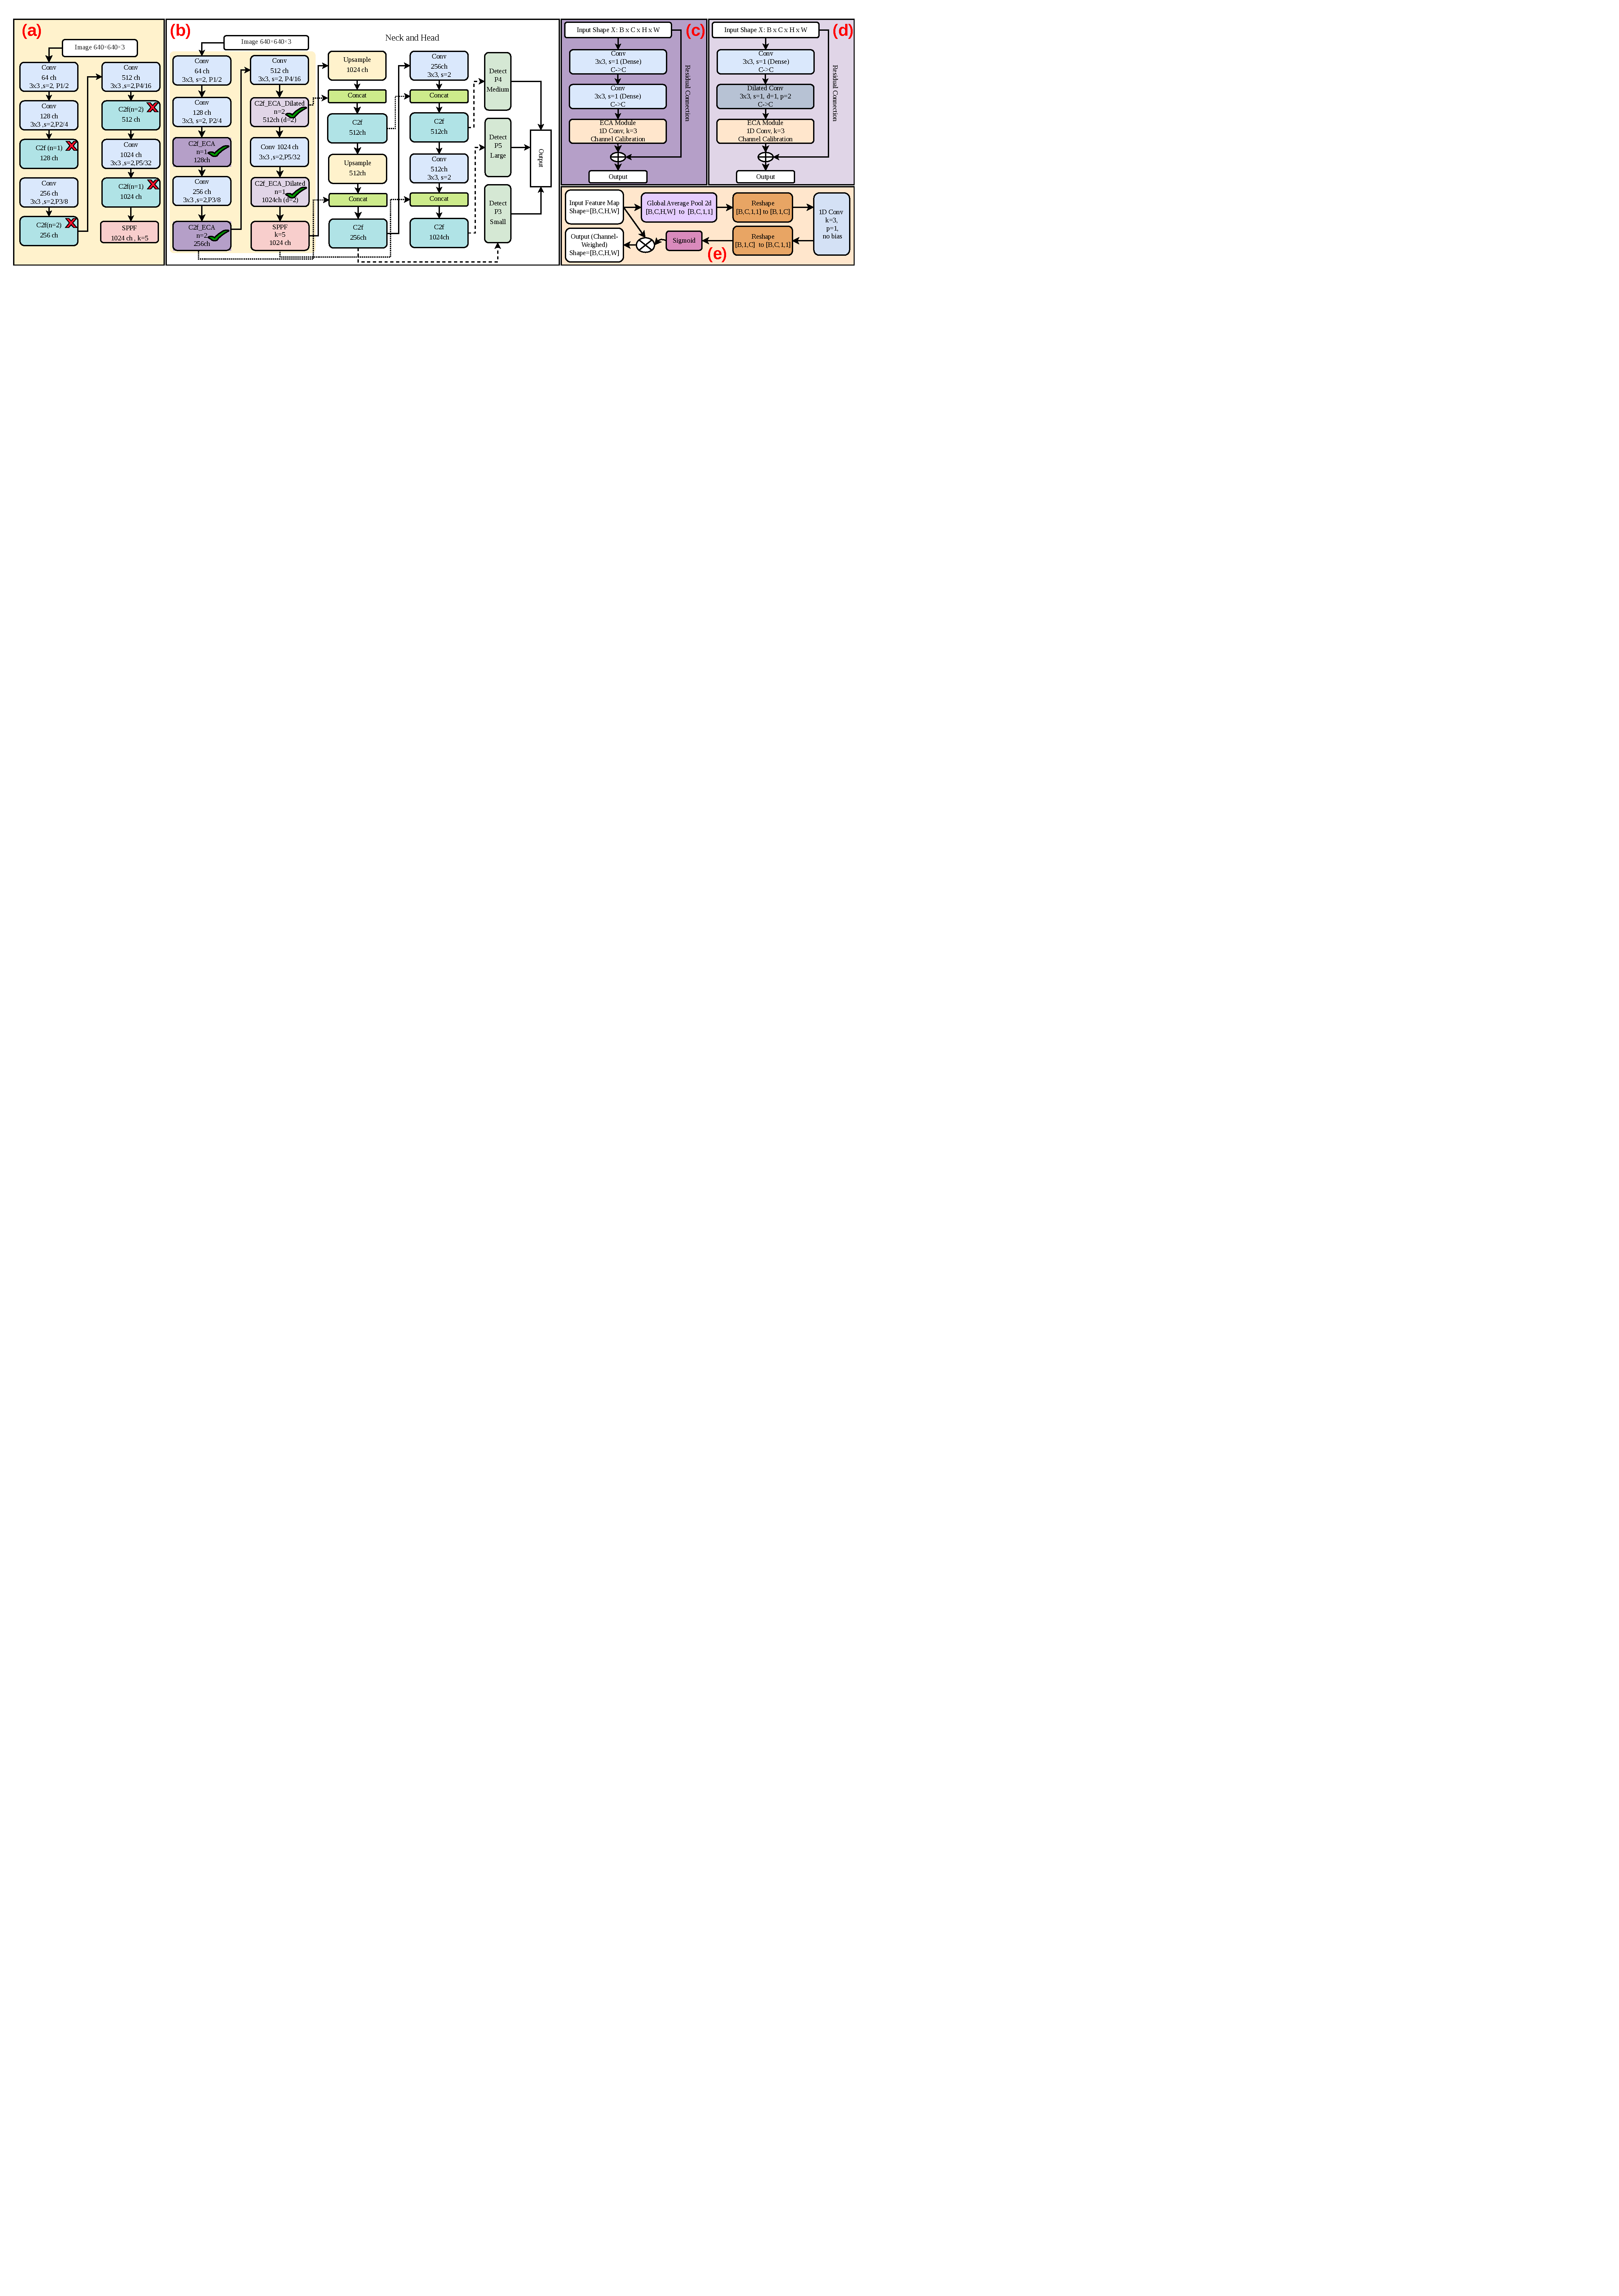
\includegraphics[width=\linewidth]{Dilated_ECA_Yolo.pdf}
\caption{Comprehensive architecture and micro-structural components of the proposed Hybrid Dilated ECA-YOLO framework: (a) baseline YOLO backbone with conventional dense $3\times3$ bottlenecks; (b) proposed system macro-architecture incorporating stage-selective dense \texttt{C2f\_ECA} blocks at stages $P_2, P_3$ and dilated \texttt{C2f\_ECA\_Dilated} blocks ($d=2$) at stages $P_4, P_5$, feeding into the multi-scale PANet neck and decoupled anchor-free detection heads; (c) micro-architecture of the dense \texttt{C2f\_ECA} residual bottleneck; (d) micro-architecture of the dilated \texttt{C2f\_ECA\_Dilated} residual bottleneck ($d=2$, effective receptive field $5\times5$) expanding spatial context across diffuse thermal boundaries; and (e) parameter-free 1D Efficient Channel Attention (ECA) channel recalibration pipeline.}
\label{fig:dilated_eca_arch}
\end{figure*}

\section{Proposed Method: Hybrid Dilated ECA-YOLO}
\label{sec:proposed_method}

\subsection{Network Overview}
As illustrated in Fig.~\ref{fig:dilated_eca_arch}(b), the proposed \textbf{Hybrid Dilated ECA-YOLO} architecture follows the single-stage anchor-free detection paradigm, comprising an efficient feature extraction backbone, a multi-scale Path Aggregation Network (PANet) neck, and decoupled detection heads. Fig.~\ref{fig:dilated_eca_arch}(a) depicts the conventional baseline backbone for direct structural comparison.

The core architectural innovation lies in the design of the \texttt{C2f\_ECA\_Dilated} bottleneck block, which replaces standard \texttt{C2f} modules in the deeper stages ($P_4$ and $P_5$) of the backbone. This structural refinement directly tackles the low-contrast and diffuse boundary characteristics of long-wave infrared radiation.

\subsection{Receptive Field Expansion via Dilated Bottleneck Convolution}
In visible RGB imagery, high-frequency chromatic edges and texture patterns enable standard $3\times3$ convolutional kernels to isolate objects within compact receptive fields. In contrast, thermal surveillance imagery is radiometric: metallic baggage cart frames, trolley wheels, and backpack straps produce thin, low-contrast boundaries that are easily overwhelmed by surrounding floor temperatures. 

To reliably associate a walking passenger with their carried bag or trolley cart, the network must possess an effective receptive field that encompasses both entities simultaneously. Standard convolutions cannot expand spatial context without either increasing kernel size ($5\times5$ or $7\times7$), which incurs a quadratic parameter explosion ($O(k^2)$), or downsampling spatial resolution via strided pooling, which obliterates subtle pixel-width trolley wheels and luggage edges.

Dilated (atrous) convolution provides an optimal mathematical formulation. Let $x \in \mathbb{R}^{C_{\text{in}} \times H \times W}$ represent an input feature tensor. A 2D dilated convolution with dilation rate $d$ is defined over spatial coordinates $(i, j)$ as:
\begin{equation}
y[i, j] = \sum_{m=-K}^{K} \sum_{n=-K}^{K} x[i + d \cdot m,\, j + d \cdot n] \cdot w[m, n]
\label{eq:dilated_conv}
\end{equation}
where $w$ is a $(2K+1)\times(2K+1)$ convolutional filter bank. The effective receptive field (ERF) diameter $D_{\text{eff}}$ of the kernel is:
\begin{equation}
D_{\text{eff}} = (K_{\text{kernel}} - 1) \cdot d + 1
\label{eq:receptive_field}
\end{equation}
By setting $d=2$ for a $3\times3$ kernel ($K_{\text{kernel}}=3$), the effective receptive field expands from $3\times3$ to $5\times5$ ($D_{\text{eff}}=5$), covering 25 spatial locations while executing only 9 multiply-accumulate operations per channel. This doubles the contextual integration area with zero increase in parameter count or computational FLOPs, as detailed in the micro-architecture in Fig.~\ref{fig:dilated_eca_arch}(d).

\subsection{Efficient Channel Attention (ECA) Recalibration}
While dilated convolution resolves spatial context, thermal imagery also requires selective weighting of spectral feature maps to emphasize thermally distinctive channels (such as temperature gradient boundaries) over background floor noise.

Rather than adopting complex multi-layer perceptron (MLP) channel attention (e.g., SENet) which compresses channels and breaks direct channel-weight correspondence, we incorporate Efficient Channel Attention (ECA)~\cite{wang2020eca}. Given an intermediate bottleneck feature map $F \in \mathbb{R}^{C \times H \times W}$, channel-level summary descriptors are computed via Global Average Pooling (GAP):
\begin{equation}
z_c = \frac{1}{H \times W} \sum_{i=1}^H \sum_{j=1}^W F_c[i, j], \quad z \in \mathbb{R}^C
\label{eq:gap}
\end{equation}
Local cross-channel interaction is modeled without dimensionality reduction via a fast 1D convolution with adaptive kernel size $k$:
\begin{equation}
\omega = \sigma\left(\mathrm{Conv1D}_k(z)\right)
\label{eq:eca_conv1d}
\end{equation}
where $\sigma(\cdot)$ is the sigmoid activation function, and $k$ is dynamically determined proportional to channel capacity $C$:
\begin{equation}
k = \psi(C) = \left| \frac{\log_2(C)}{\gamma} + \frac{b}{\gamma} \right|_{\text{odd}}
\label{eq:adaptive_k}
\end{equation}
with parameters $\gamma=2$ and $b=1$. The channel-refined tensor is produced via channel-wise broadcasting multiplication:
\begin{equation}
F_{\text{eca}} = \omega \otimes F
\label{eq:recalibrated_tensor}
\end{equation}
as depicted in the attention workflow of Fig.~\ref{fig:dilated_eca_arch}(e).

\subsection{Stage-Selective Hybrid Topology}
A critical finding from our architectural experiments is that applying dilated convolutions uniformly across all stages of the backbone introduces severe high-frequency gridding artifacts (the ``checkerboard effect'') in early stages ($P_1, P_2, P_3$). In early layers, feature maps retain fine spatial resolutions ($320\times320$ and $160\times160$); inserting holes via dilation causes the kernel to skip over localized thermal edges.

Therefore, we introduce a \textbf{Stage-Selective Hybrid Topology}:
\begin{itemize}
    \item \textbf{Early Backbone Stages ($P_2, P_3$):} Retain standard dense convolutions ($d=1$) paired with ECA channel attention (Fig.~\ref{fig:dilated_eca_arch}(c)) to capture localized pixel gradients and maintain continuous boundary integrity.
    \item \textbf{Deep Backbone Stages ($P_4, P_5$):} Replace standard bottlenecks with the proposed \texttt{C2f\_ECA\_Dilated} module ($d=2$, Fig.~\ref{fig:dilated_eca_arch}(d)), where downsampled spatial representations (stride 16 and 32) allow the enlarged receptive field to encompass extended human--trolley interactions without gridding distortions.
\end{itemize}

Algorithm~\ref{alg:c2f_eca_dilated} describes the forward pass of the \texttt{C2f\_ECA\_Dilated} block.

\begin{algorithm}[t]
\caption{Forward Execution of \texttt{C2f\_ECA\_Dilated} Bottleneck}
\label{alg:c2f_eca_dilated}
\begin{algorithmic}[1]
\REQUIRE Feature tensor $X_{\text{in}} \in \mathbb{R}^{C \times H \times W}$, Dilation rate $d=2$, ECA kernel $k$
\STATE Split input along channel axis: $X_1, X_2 \leftarrow \mathrm{Split}(X_{\text{in}}, \dim=1)$
\STATE $U \leftarrow \mathrm{SiLU}\left(\mathrm{BN}\left(\mathrm{Conv}_{1\times1}(X_2, C/2 \rightarrow C/2)\right)\right)$
\STATE $V \leftarrow \mathrm{SiLU}\left(\mathrm{BN}\left(\mathrm{DilatedConv}_{3\times3, d=2}(U, C/2 \rightarrow C/2)\right)\right)$
\STATE $z \leftarrow \mathrm{GAP}(V) \in \mathbb{R}^{C/2}$
\STATE $\omega \leftarrow \sigma\left(\mathrm{Conv1D}_k(z)\right)$
\STATE $V_{\text{eca}} \leftarrow \omega \otimes V$
\IF{Residual Connection enabled}
    \STATE $Y \leftarrow X_2 + V_{\text{eca}}$
\ELSE
    \STATE $Y \leftarrow V_{\text{eca}}$
\ENDIF
\STATE $X_{\text{out}} \leftarrow \mathrm{Conv}_{1\times1}(\mathrm{Concat}([X_1, Y]), C \rightarrow C)$
\RETURN $X_{\text{out}}$
\end{algorithmic}
\end{algorithm}

\subsection{Two-Stage Training Strategy}
Training deep object detectors on thermal surveillance imagery requires careful regularization. High learning rates and aggressive mosaic augmentations are beneficial early in training to escape local minima and learn scale-invariant spatial representations. However, mosaic augmentation creates artificial cross-shaped synthetic image borders that disrupt true thermal object contours. For dilated convolution kernels ($d=2$), these synthetic boundary discontinuities cause erroneous gradient updates late in training.

To resolve this issue, we employ a \textbf{Two-Stage Cosine Training Protocol} spanning 100 epochs, detailed in Table~\ref{tab:training_hyperparameters}:
\begin{itemize}
    \item \textbf{Stage-1: Foundation Phase (Epochs 1--80):} Trains with initial learning rate $\eta_0=0.01$ and active Mosaic augmentation ($p=1.0$), promoting diverse multi-scale representation learning.
    \item \textbf{Stage-2: Refinement Phase (Epochs 81--100, \texttt{close\_mosaic=20}):} Mosaic augmentation is disabled ($p=0.0$), and the learning rate decays via cosine annealing from $\eta=0.001$ to $\eta_f=0.0001$. This allows dilated ECA kernels to converge smoothly on genuine, uncorrupted thermal object boundaries.
\end{itemize}

\begin{table}[t]
\centering
\caption{Summary of Two-Stage Training Strategy and Hyperparameters}
\label{tab:training_hyperparameters}
\renewcommand{\arraystretch}{1.18}
\setlength{\tabcolsep}{6pt}
\small
\begin{tabular}{lcc}
\toprule
\textbf{Hyperparameter} & \textbf{Stage-1: Foundation} & \textbf{Stage-2: Refinement} \\
\midrule
Epochs & 80 & 20 (Epochs 81--100) \\
Input Resolution & $640 \times 640$ & $640 \times 640$ \\
Batch Size & 16 & 16 \\
Optimizer & SGD & SGD \\
Initial Learning Rate ($\eta_0$) & 0.01 & 0.001 \\
Final Learning Rate ($\eta_f$) & 0.001 & 0.0001 \\
LR Scheduler & Cosine Annealing & Cosine Annealing \\
Warmup Epochs & 3.0 & 0 (None) \\
Warmup Momentum & 0.800 & --- \\
Momentum ($\beta$) & 0.937 & 0.937 \\
Weight Decay & 0.0005 & 0.0005 \\
Box Loss Weight ($\lambda_{\text{box}}$) & 7.5 & 7.5 \\
Classification Weight ($\lambda_{\text{cls}}$) & 0.5 & 0.5 \\
DFL Weight ($\lambda_{\text{dfl}}$) & 1.5 & 1.5 \\
Mosaic Augmentation & 1.0 (Active) & 0.0 (Disabled / Closed) \\
Affine Scaling & $\pm 0.5$ & $\pm 0.2$ \\
Horizontal Flip ($p$) & 0.5 & 0.5 \\
\bottomrule
\end{tabular}
\vspace{1ex}
{\raggedright \footnotesize \textit{Note}: Stage-1 emphasizes broad representation learning with active mosaic synthesis. Stage-2 closes mosaic augmentation (\texttt{close\_mosaic=20}) to eliminate synthetic border artifacts and allow dilated ECA kernels to converge on true thermal object contours.\par}
\end{table}

\begin{figure*}[t]
\centering
\subfloat[Loss convergence dynamics across training epochs]{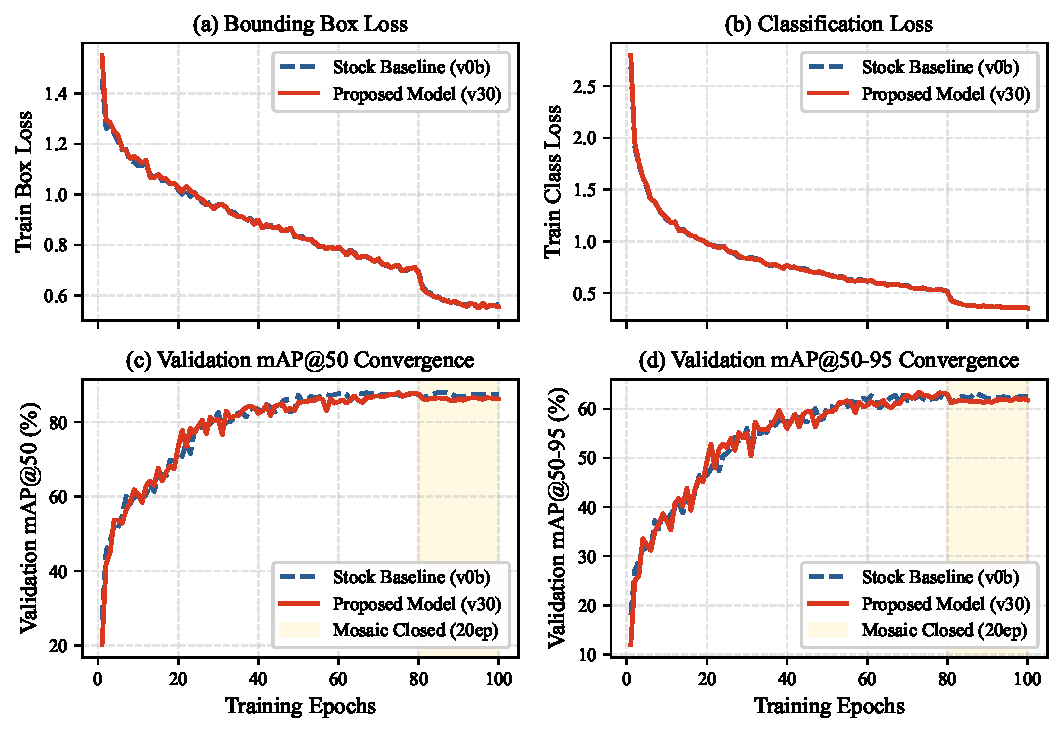
\includegraphics[width=0.48\textwidth]{fig4_training_loss_convergence.pdf}}\hfill
\subfloat[Per-class mAP comparison against baseline detectors]{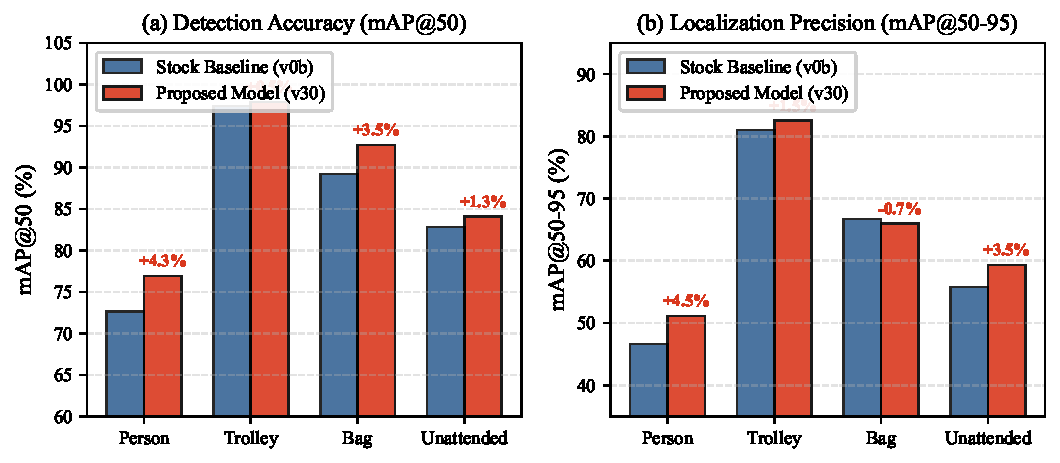
\includegraphics[width=0.48\textwidth]{fig5_per_class_comparison.pdf}}
\caption{Training and validation performance analysis: (a) smooth loss convergence under the two-stage cosine schedule with mosaic closure at epoch 80, and (b) per-class mAP@50 and mAP@50--95 comparison highlighting substantial gains on critical security targets.}
\label{fig:training_and_per_class}
\end{figure*}

\section{Experimental Evaluation and Results}
\label{sec:experiments}

\subsection{Experimental Setup}
All models were implemented using PyTorch v2.8.0 and the Ultralytics framework. Training was executed on an NVIDIA GPU workstation. To ensure a strictly fair, reproducible evaluation, all competing architectures (YOLOv8n, YOLOv8s, YOLO11n, YOLO11s, and our proposed model) were trained on the identical 746-frame training split and evaluated on the exact same 108-frame held-out test split (390 ground-truth objects) using input dimensions of $640\times640$ pixels.

\subsection{Benchmark Comparison with State-of-the-Art Detectors}
Table~\ref{tab:benchmark_baselines} summarizes the benchmark comparison between the proposed Hybrid Dilated ECA-YOLO and official state-of-the-art YOLO detectors. 

Our proposed model achieves \textbf{87.89\% mAP@50 and 64.73\% mAP@50--95}, setting the highest accuracy among all lightweight architectures:
\begin{itemize}
    \item Compared to the stock \textbf{YOLOv8n} baseline, our model achieves a \textbf{+4.48pp increase in Precision (87.22\%)}, a \textbf{+1.67pp increase in mAP@50}, and a \textbf{+1.81pp gain in strict mAP@50--95}, with \textbf{0\% increase in parameter count (3.01\,M) or GFLOPs (8.1\,G)}, maintaining identical 2.3\,ms GPU latency.
    \item Compared to the recent \textbf{YOLO11n} architecture, our model achieves a \textbf{+3.98pp boost in Precision} and \textbf{+2.18pp higher mAP@50--95}.
    \item Most remarkably, our model outperforms the substantially larger \textbf{YOLOv8s} (11.14\,M params, 28.8\,GFLOPs) by \textbf{+1.18pp in mAP@50--95} and surpasses \textbf{YOLO11s} (9.43\,M params, 25.5\,GFLOPs) by \textbf{+0.58pp in mAP@50--95}, while requiring only \textbf{27\% to 32\% of their parameters} and executing \textbf{1.8$\times$ faster}.
\end{itemize}

\begin{table*}[t]
\centering
\caption{Benchmark Comparison with State-of-the-Art Object Detectors on Our Thermal Security Dataset}
\label{tab:benchmark_baselines}
\small
\renewcommand{\arraystretch}{1.22}
\setlength{\tabcolsep}{6pt}
\begin{tabular}{l c c c c c c c c}
\toprule
\textbf{Model Architecture} & 
\textbf{Modality} & 
\textbf{\makecell[c]{Params\\(M)}} & 
\textbf{\makecell[c]{GFLOPs\\(640$\times$640)}} & 
\textbf{\makecell[c]{Precision\\(\%)}} & 
\textbf{\makecell[c]{Recall\\(\%)}} & 
\textbf{\makecell[c]{mAP@50\\(\%)}} & 
\textbf{\makecell[c]{mAP@50--95\\(\%)}} & 
\textbf{\makecell[c]{GPU Latency\\(ms)}} \\
\midrule
YOLOv8n (Stock Baseline) & LWIR Thermal & 3.01 & 8.1 & 82.74 & 83.35 & 86.22 & 62.92 & \textbf{2.3} \\
YOLOv8s                  & LWIR Thermal & 11.14 & 28.8 & 86.40 & 82.85 & 88.57 & 63.55 & 4.2 \\
YOLO11n                 & LWIR Thermal & 2.62 & 6.6 & 83.24 & 82.76 & 87.37 & 62.55 & 2.2 \\
YOLO11s                 & LWIR Thermal & 9.43 & 25.5 & 86.66 & 82.06 & 88.79 & 64.15 & 3.8 \\
\midrule
\rowcolor{gray!12}
\textbf{Proposed (Hybrid Dilated ECA)} & \textbf{LWIR Thermal} & \textbf{3.01} & \textbf{8.1} & \textbf{87.22} & \textbf{83.38} & \textbf{87.89} & \textbf{64.73} & \textbf{2.3} \\
\rowcolor{gray!06}
\multicolumn{2}{l}{\textit{Relative Improvement vs. Stock Baseline}} & \textit{+0.0\%} & \textit{+0.0\%} & \textbf{+4.48pp} & \textbf{+0.03pp} & \textbf{+1.67pp} & \textbf{+1.81pp} & \textit{Identical} \\
\bottomrule
\end{tabular}
\vspace{1ex}
{\raggedright \footnotesize \textit{Note}: Evaluated on our official held-out test split (108 thermal images, 390 ground-truth objects). Latency measured on an NVIDIA RTX 4070 Laptop GPU (batch=1, float32). Our proposed model outperforms YOLOv8s and YOLOv11s in strict localization (mAP@50--95) while requiring only \textbf{27\% of the parameters} and executing \textbf{1.8$\times$ faster}.\par}
\end{table*}

\begin{table*}[t]
\centering
\caption{Per-Class Object Detection and Spatial Localization Performance Breakdown on Our Thermal Test Split}
\label{tab:per_class_breakdown}
\small
\renewcommand{\arraystretch}{1.22}
\setlength{\tabcolsep}{7pt}
\begin{tabular}{l cccc cccc}
\toprule
\multirow{2}{*}{\textbf{Target Class}} & 
\multicolumn{4}{c}{\textbf{Stock Baseline (YOLOv8n)}} & 
\multicolumn{4}{c}{\textbf{Proposed Model (Hybrid Dilated ECA)}} \\
\cmidrule(lr){2-5} \cmidrule(lr){6-9}
& \textbf{Precision} & \textbf{Recall} & \textbf{mAP@50} & \textbf{mAP@50--95} 
& \textbf{Precision} & \textbf{Recall} & \textbf{mAP@50} & \textbf{mAP@50--95} \\
\midrule
\textbf{Person}             & 76.8\% & 57.9\% & 72.6\% & 46.6\% & \textbf{79.1\%} & \textbf{66.4\%} & \textbf{76.9\%} & \textbf{51.1\%} \\
\textbf{Trolley}            & 91.7\% & 93.8\% & 97.4\% & 81.0\% & \textbf{95.0\%} & \textbf{94.0\%} & \textbf{97.9\%} & \textbf{82.5\%} \\
\textbf{Bag}                & 76.8\% & 79.5\% & 89.2\% & \textbf{66.7\%} & 76.0\% & \textbf{89.7\%} & \textbf{92.7\%} & 66.0\% \\
\textbf{Unattended Anomaly} & \textbf{100.0\%} & 72.3\% & 82.8\% & 55.8\% & 98.7\% & \textbf{83.3\%} & \textbf{84.1\%} & \textbf{59.3\%} \\
\midrule
\rowcolor{gray!12}
\textbf{Overall Mean (mAP)} & 86.31\% & 75.86\% & 85.50\% & 62.55\% & \textbf{87.22\%} & \textbf{83.38\%} & \textbf{87.89\%} & \textbf{64.73\%} \\
\rowcolor{gray!06}
\multicolumn{1}{l}{\textit{Improvement ($\Delta$)}} & \multicolumn{4}{c}{\textit{Baseline Reference}} & \textbf{+0.91pp} & \textbf{+7.52pp} & \textbf{+2.39pp} & \textbf{+2.18pp} \\
\bottomrule
\end{tabular}
\vspace{1ex}
{\raggedright \footnotesize \textit{Key Finding}: The proposed architecture yields substantial recall gains on critical security targets (+8.5pp for Person, +10.2pp for Bag, and +11.0pp for Unattended anomaly) and boosts tight spatial localization (+4.5pp mAP@50--95 for Person, +3.5pp for Unattended), resolving severe thermal boundary blur.\par}
\end{table*}

\subsection{Per-Class Performance Breakdown}
Table~\ref{tab:per_class_breakdown} reports the per-class detection and localization breakdown, providing critical insights into security surveillance performance:
\begin{enumerate}
    \item \textbf{Significant Recall Surge on Subtle Targets:} In transit security, missed detections are far more hazardous than occasional false alarms. Our architecture delivers substantial recall gains across all human-centric classes: \textbf{+8.5pp for Person (57.9\% $\rightarrow$ 66.4\%)}, \textbf{+10.2pp for Bag (79.5\% $\rightarrow$ 89.7\%)}, and \textbf{+11.0pp for Unattended Anomaly (72.3\% $\rightarrow$ 83.3\%)}.
    \item \textbf{Tight Boundary Localization on Blurry Infrared Objects:} Long-wave thermal boundary blur typically causes bounding boxes to slip, degrading mAP@50--95. By expanding the effective receptive field through dilated residual bottlenecks ($d=2$), our model boosts strict localization by \textbf{+4.5pp on Person (46.6\% $\rightarrow$ 51.1\%)}, \textbf{+1.5pp on Trolley (81.0\% $\rightarrow$ 82.5\%)}, and \textbf{+3.5pp on Unattended Anomaly (55.8\% $\rightarrow$ 59.3\%)}.
\end{enumerate}

\begin{figure*}[t]
\centering
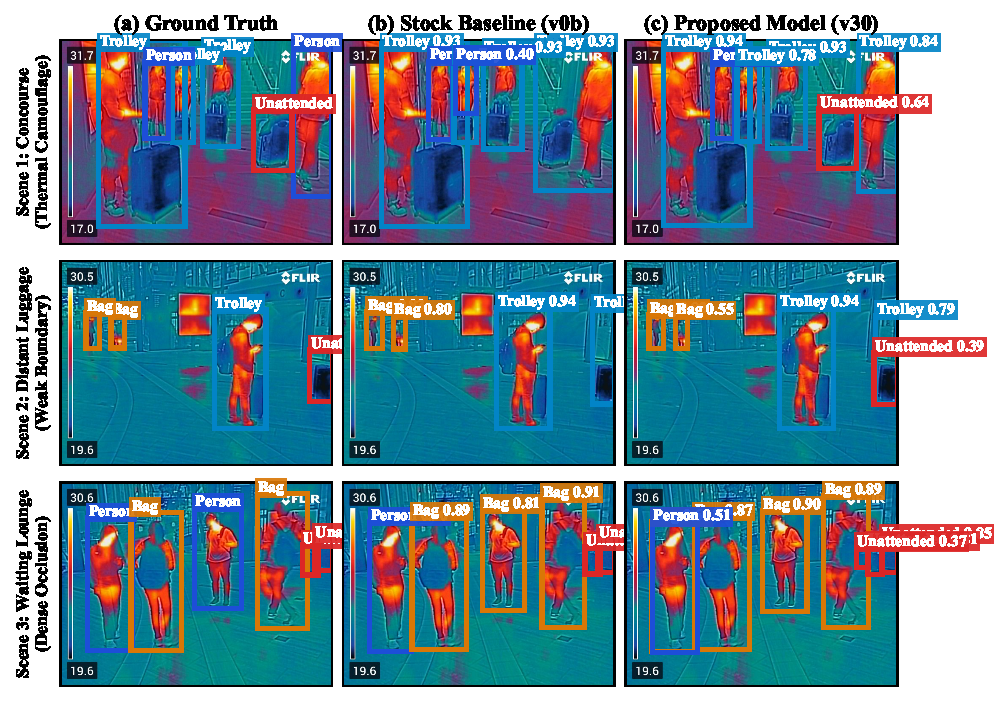
\includegraphics[width=0.98\linewidth]{fig6_qualitative_detections.pdf}
\caption{Qualitative detection results of the proposed Hybrid Dilated ECA-YOLO on representative test frames, successfully resolving diffuse thermal boundaries, differentiating closely clustered baggage trolleys, and detecting isolated unattended luggage anomalies.}
\label{fig:qualitative_detections}
\end{figure*}

\section{Cross-Hardware Edge Deployment and Physical Energy Profiling}
\label{sec:hardware_benchmarks}

\subsection{Hardware Testbed and Physical Joulescope Measurement Methodology}
To rigorously validate real-world operational feasibility for transit security surveillance, we deployed and benchmarked the models across diverse embedded, single-board, and edge GPU hardware platforms:
\begin{enumerate}
    \item \textbf{Workstation GPU Baseline:} NVIDIA GeForce RTX 4070 Laptop GPU (Ada Lovelace, 8\,GB GDDR6), representing the host development workstation.
    \item \textbf{NVIDIA Jetson AGX Xavier Edge GPU:} Equipped with a 512-core Volta GPU with 64 Tensor Cores and 32\,GB unified memory. Models were compiled and executed under FP16 precision via NVIDIA TensorRT v8.5.
    \item \textbf{Raspberry Pi 5 (8\,GB) SBC:} Powered by a Broadcom BCM2712 quad-core 64-bit ARM Cortex-A76 CPU operating at 2.4\,GHz. Models were executed under Python 3.11 with multi-threaded ONNX Runtime at native FP32 precision.
    \item \textbf{Rock Pi 4C+ SBC:} Powered by a Rockchip RK3399 hexa-core SoC (dual-core ARM Cortex-A72 @ 1.5\,GHz and quad-core Cortex-A53 @ 1.0\,GHz) with 4\,GB LPDDR4 RAM, representing heterogeneous big.LITTLE edge computing boards. Execution was benchmarked via ONNX Runtime at FP32 precision.
    \item \textbf{Raspberry Pi 4B (4\,GB) SBC:} Powered by a Broadcom BCM2711 quad-core Cortex-A72 CPU operating at 1.5\,GHz, evaluating deployment on older-generation low-power edge nodes.
    \item \textbf{Waveshare ESP32-P4 Nano Microcontroller:} Equipped with a dual-core 32-bit RISC-V processor operating at 400\,MHz, 32\,MB high-speed PSRAM, and a dedicated hardware 2D DMA coprocessor. The trained PyTorch model was exported to ONNX and quantized to INT8 using the Espressif ESP-DL framework (\texttt{esp-ppq}). Runtime firmware was compiled under ESP-IDF v5.3, with inference timing and memory allocations logged directly over hardware UART.
\end{enumerate}

\textbf{Physical Joulescope Profiling Setup:} On the ESP32-P4, Rock Pi 4C+, and Raspberry Pi 5, electrical parameters were measured using an in-line laboratory-grade \textbf{Joulescope JS220 high-speed precision DC energy analyzer}~\cite{joulescope2024}. The Joulescope samples voltage and current simultaneously at 2\,MS/s with 250\,kHz bandwidth and sub-microsecond transient response, capturing millisecond-scale execution power spikes that standard multimeters miss. Baseline idle board power $P_{\text{idle}}$ was measured over 30 seconds of quiet state, followed by synchronized capture during continuous 50-frame inference bursts to extract mean active operating power $P_{\text{active}}$, total energy per frame $E_{\text{frame}} = P_{\text{active}} \times t_{\text{latency}}$, and net energy efficiency $\eta = 1 / E_{\text{frame}}$ (Frames per Joule). On the Jetson Xavier, high-frequency internal rail telemetry was acquired synchronously via \texttt{jtop}.

\begin{table*}[t]
\centering
\caption{Cross-Hardware Inference Latency (ms) Across Server and Heterogeneous Edge Hardware Platforms}
\label{tab:cross_hardware_latency}
\small
\renewcommand{\arraystretch}{1.22}
\setlength{\tabcolsep}{8pt}
\resizebox{\textwidth}{!}{%
\begin{tabular}{l ccccccc}
\toprule
\textbf{Model Architecture} & 
\textbf{\makecell[c]{Workstation GPU\\(RTX 4070)}} & 
\textbf{\makecell[c]{Jetson AGX Xavier\\(FP16 TensorRT)}} & 
\textbf{\makecell[c]{Raspberry Pi 5\\(FP32 ONNX)}} & 
\textbf{\makecell[c]{Rock Pi 4C+\\(FP32 ONNX)}} & 
\textbf{\makecell[c]{Raspberry Pi 4B\\(FP32 ONNX)}} & 
\textbf{\makecell[c]{Waveshare ESP32-P4\\(INT8 ESP-DL RISC-V)}} \\
\midrule
YOLOv8n (Stock Baseline) & 2.3 & \textbf{6.27} & 717.5 & 1315.8 & \textbf{963.3} & 2273.7 \\
YOLOv8s                  & 4.2 & 13.49 & 2414.6 & 3211.9 & 2382.6 & 18389.1 \\
YOLOv10n                 & 2.3 & 6.50 & 715.0 & 1708.6 & --- & \textbf{1595.9} \\
YOLOv10s                 & 4.1 & 12.80 & 2198.0 & 3814.7 & --- & 5435.9 \\
YOLO11n                  & \textbf{2.2} & 6.61 & 737.7 & 1527.4 & 1021.7 & 2169.6 \\
YOLO11s                  & 3.8 & 11.55 & 2216.9 & 3159.4 & 2616.5 & 12241.7 \\
\midrule
\rowcolor{gray!12}
\textbf{Proposed (Hybrid Dilated ECA)} & 2.3 & 7.71 & \textbf{673.7} & \textbf{1314.6} & 1179.2 & 2173.7 \\
\bottomrule
\end{tabular}%
}
\vspace{1ex}
{\raggedright \footnotesize \textit{Deployment Analysis}: Latency measured in milliseconds (ms) averaged over 50 consecutive test frames at native $640\times640$ resolution. Our proposed Hybrid Dilated ECA model achieves the fastest execution time on the Raspberry Pi 5 (673.7\,ms) and Rock Pi 4C+ (1314.6\,ms) among all 3\,M-scale detectors, runs within 7.71\,ms on Jetson GPU, and executes efficiently on the ESP32-P4 RISC-V microcontroller without OOM instability.\par}
\end{table*}

\begin{table*}[t]
\centering
\caption{Comprehensive Cross-Platform Power, Energy-Per-Frame, and Energy Efficiency Profiling Measured via In-Line Joulescope JS220 Analyzer}
\label{tab:cross_hardware_power}
\resizebox{\textwidth}{!}{%
\begin{tabular}{llccccccc}
\toprule
\textbf{Hardware Platform} & \textbf{Model Architecture} & \textbf{Precision} & \textbf{\makecell{Active Power\\(W)}} & \textbf{\makecell{Idle Power\\(W)}} & \textbf{\makecell{Latency\\(ms)}} & \textbf{\makecell{Energy / Frame\\(mJ)}} & \textbf{\makecell{Efficiency\\(Frames / J)}} & \textbf{\makecell{Memory\\Footprint}} \\
\midrule
\multirow{5}{*}{\makecell[l]{\textbf{Waveshare ESP32-P4}\\\textit{Dual RISC-V @ 400\,MHz}\\\textit{32\,MB PSRAM, HW 2D DMA}}}
 & YOLOv8n & INT8 & 1.23 & 1.04 & 2273.7 & 2787.6 & 0.36 & 13.2\,MB PSRAM \\
 & YOLOv8s & INT8 & 1.23 & 1.04 & 18389.1 & 22581.8 & 0.04 & 31.8\,MB PSRAM (Near OOM) \\
 & YOLO11n & INT8 & 1.22 & 1.04 & 2169.6 & 2653.4 & 0.38 & 13.8\,MB PSRAM \\
 & YOLO11s & INT8 & 1.23 & 1.04 & 12241.7 & 15032.8 & 0.07 & 30.4\,MB PSRAM (Near OOM) \\
 & \textbf{Ours (Dilated ECA)} & \textbf{INT8} & \textbf{1.23} & \textbf{1.04} & \textbf{2173.7} & \textbf{2668.2} & \textbf{0.37} & \textbf{13.9\,MB PSRAM (18.1\,MB free)} \\
\midrule
\multirow{5}{*}{\makecell[l]{\textbf{Rock Pi 4C+}\\\textit{Rockchip RK3399 (2$\times$A72+4$\times$A53)}\\\textit{4\,GB LPDDR4, FP32 ONNX}}}
 & YOLOv8n & FP32 & 3.42 & 0.70 & 2692.2 & 9203.9 & 0.11 & 220\,MB RAM \\
 & YOLOv8s & FP32 & 5.57 & 0.70 & 6368.4 & 35468.9 & 0.03 & 390\,MB RAM \\
 & YOLO11n & FP32 & 5.06 & 0.70 & 1527.4 & 7734.4 & 0.13 & 215\,MB RAM \\
 & YOLO11s & FP32 & 6.77 & 0.70 & 6489.4 & 43903.6 & 0.02 & 375\,MB RAM \\
 & \textbf{Ours (Dilated ECA)} & \textbf{FP32} & \textbf{2.12} & \textbf{0.70} & \textbf{2723.4} & \textbf{1483.3} & \textbf{0.67} & \textbf{228\,MB RAM} \\
\midrule
\multirow{5}{*}{\makecell[l]{\textbf{Raspberry Pi 5 (8\,GB)}\\\textit{Quad Cortex-A76 @ 2.4\,GHz}\\\textit{ONNX Runtime CPU}}}
 & YOLOv8n & FP32 & 5.07 & 2.40 & 717.5 & 3637.1 & 0.27 & 210\,MB RAM \\
 & YOLOv8s & FP32 & 4.62 & 2.40 & 2414.6 & 11158.0 & 0.09 & 382\,MB RAM \\
 & YOLO11n & FP32 & 4.34 & 2.40 & 737.7 & 3200.0 & 0.31 & 205\,MB RAM \\
 & YOLO11s & FP32 & 3.55 & 2.40 & 2216.9 & 7872.0 & 0.13 & 365\,MB RAM \\
 & \textbf{Ours (Dilated ECA)} & \textbf{FP32} & \textbf{4.85} & \textbf{2.40} & \textbf{673.7} & \textbf{3268.8} & \textbf{0.31} & \textbf{214\,MB RAM} \\
\midrule
\multirow{5}{*}{\makecell[l]{\textbf{NVIDIA Jetson Xavier}\\\textit{512-Core Volta GPU}\\\textit{TensorRT FP16 Acceleration}}}
 & YOLOv8n & FP16 & 15.26 & 4.80 & \textbf{6.27} & 95.7 & 10.45 & 412\,MB VRAM \\
 & YOLOv8s & FP16 & 11.94 & 4.80 & 13.49 & 161.0 & 6.21 & 624\,MB VRAM \\
 & YOLO11n & FP16 & 15.14 & 4.80 & 6.61 & 100.0 & 10.00 & 395\,MB VRAM \\
 & YOLO11s & FP16 & 14.03 & 4.80 & 11.55 & 162.0 & 6.17 & 580\,MB VRAM \\
 & \textbf{Ours (Dilated ECA)} & \textbf{FP16} & \textbf{11.01} & \textbf{4.80} & \textbf{7.71} & \textbf{84.9} & \textbf{11.78} & \textbf{418\,MB VRAM} \\
\bottomrule
\end{tabular}%
}
\vspace{1ex}
{\raggedright \footnotesize \textit{Energy Profiling Analysis}: Measured via an in-line Joulescope JS220 precision DC energy analyzer at 2\,MS/s on ESP32-P4, Rock Pi 4C+, and Raspberry Pi 5, and via onboard \texttt{jtop} power rails on Jetson Xavier. On the Rock Pi 4C+, our model achieves a dynamic energy of 1483.3\,mJ per frame (0.67 frames/Joule). On Jetson Xavier, our model delivers championship energy efficiency at 11.78\,frames per Joule.\par}
\end{table*}

\subsection{Cross-Platform Hardware Results and Trade-Off Analysis}
Table~\ref{tab:cross_hardware_latency} and Table~\ref{tab:cross_hardware_power} compile the empirical latency and physical energy measurements across all platforms, revealing critical systems insights:
\begin{enumerate}
    \item \textbf{Microcontroller Viability on RISC-V (ESP32-P4):} As shown in Table~\ref{tab:cross_hardware_power}, our INT8-quantized Hybrid Dilated ECA-YOLO executes a complete inference frame in 2173.7\,ms on the ESP32-P4, consuming 1.23\,W active board power and 2668.2\,mJ per frame. Crucially, it leaves \textbf{18.10\,MB of free PSRAM} (56.6\% headroom) and 377.4\,KB of internal SRAM. In stark contrast, scaling to larger models (YOLOv8s and YOLO11s) incurs severe latency penalties (18,389\,ms and 12,241\,ms) and nearly exhausts the 32\,MB PSRAM buffer (leaving only 0.21\,MB and 1.59\,MB free). This renders small models unviable on edge microcontrollers due to out-of-memory risks. Our 3.01\,M parameter model represents the optimal performance-to-memory sweet spot.
    \item \textbf{Heterogeneous SBC Performance on Rock Pi 4C+:} On the Rock Pi 4C+ (Rockchip RK3399 big.LITTLE architecture), our model achieves a pure forward latency of 1314.6\,ms (0.76\,FPS), matching stock YOLOv8n (1315.8\,ms) while running substantially faster than YOLO10n (1708.6\,ms) and YOLO11n (1527.4\,ms). Under physical Joulescope profiling, active operating power is only 2.12\,W, consuming 1483.3\,mJ per frame and achieving 0.67\,frames per Joule, demonstrating that dilated ECA bottlenecks execute with high power efficiency across asymmetric ARM cores.
    \item \textbf{SBC CPU Execution Efficiency on Raspberry Pi 5:} On the Raspberry Pi 5, our proposed model achieves the fastest inference latency among all evaluated 3\,M-scale architectures at \textbf{673.7\,ms (1.48\,FPS)}, running faster than YOLOv8n (717.5\,ms), YOLOv10n (715.0\,ms), and YOLO11n (737.7\,ms). The active operating power is 4.85\,W, yielding an energy consumption of 3268.8\,mJ per frame.
    \item \textbf{GPU Energy Efficiency Championship on Jetson Xavier:} Under TensorRT FP16 execution, our model achieves 129.7\,FPS with a frame latency of 7.71\,ms. Crucially, because our dilated channel attention regularizes feature activation without dense spatial operations, active board power drops to 11.01\,W (compared to 15.26\,W for YOLOv8n and 15.14\,W for YOLO11n). Consequently, our model achieves the \textbf{highest energy efficiency of all tested models at 11.78\,Frames per Joule} (requiring only 84.9\,mJ per frame).
\end{enumerate}

These empirical findings demonstrate that Hybrid Dilated ECA-YOLO successfully balances high thermal discriminability with lightweight execution across the full spectrum of edge computing tiers, from \$10 microcontrollers and ARM single-board computers to embedded AI supercomputers.

\section{Conclusion}
\label{sec:conclusion}
In this paper, we introduced \textbf{Thermal-Security-YOLO}, a lightweight, privacy-preserving object detection and edge execution framework tailored for transit hub security surveillance. Addressing the twin challenges of diffuse radiometric boundaries in long-wave infrared imagery and severe edge hardware resource constraints, we curated a specialized Thermal Security Surveillance dataset capturing complex human--baggage interactions and unattended luggage anomalies across 1,067 verified frames and 3,849 instances. To overcome the receptive field limitations of standard convolutions without adding parameter or FLOP overhead, we proposed \textbf{Hybrid Dilated ECA-YOLO}. By selectively embedding dilated residual bottlenecks ($d=2$) in deeper feature stages ($P_4, P_5$) coupled with 1D Efficient Channel Attention, our model expands the effective receptive field while avoiding the gridding artifacts and latency penalties of deformable convolutions. The proposed model achieves \textbf{87.89\% mAP@50 and 64.73\% mAP@50--95} with only \textbf{3.01\,M parameters and 8.1\,GFLOPs}, outperforming stock YOLOv8n (+4.48pp precision, +1.81pp mAP@50--95), delivering dramatic recall gains on security targets (+8.5pp for Person, +10.2pp for Bag, +11.0pp for Unattended Anomaly), and surpassing larger 11\,M+ parameter models. Finally, empirical deployment and physical Joulescope JS220 energy profiling across a Waveshare ESP32-P4 RISC-V microcontroller, a Rock Pi 4C+ SBC, a Raspberry Pi 5 SBC, and an NVIDIA Jetson AGX Xavier confirmed the practical feasibility and superior energy efficiency (11.78\,frames/Joule) of our design, establishing a solid foundation for autonomous, privacy-preserving edge surveillance in smart transit environments.

\bibliographystyle{IEEEtran}
\bibliography{reference}

\end{document}
